\section[M3: QVTo]{M3: QVTo - Modelltransformation}
\begin{frame}{QVTo - Modelltransformation}
	\centering
	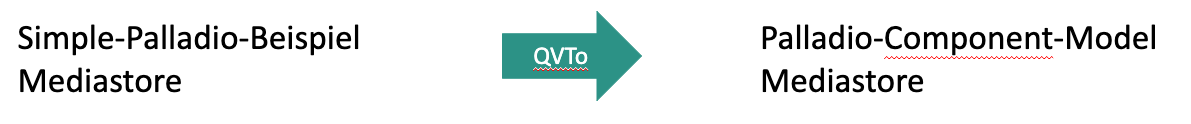
\includegraphics[height=10mm]{figures/modelltransformation.png}
	\begin{enumerate}
		\item Definieren von Eingabe-Modellen, Ausgabemodellen und Transformation zwischen diesen
		\item Probleme
		\begin{itemize}
			\item Verschiedene Modellierungen (Enum vs. Relation vs. Objekt)
			\item Vererbungshierarchien
			\item Weniger-explizite Informationen in SimplePalladio
		\end{itemize}
	\end{enumerate}
\end{frame}

\begin{frame}{Verschiedene Modellierungen (Enum vs. Objekt)}
	\centering
	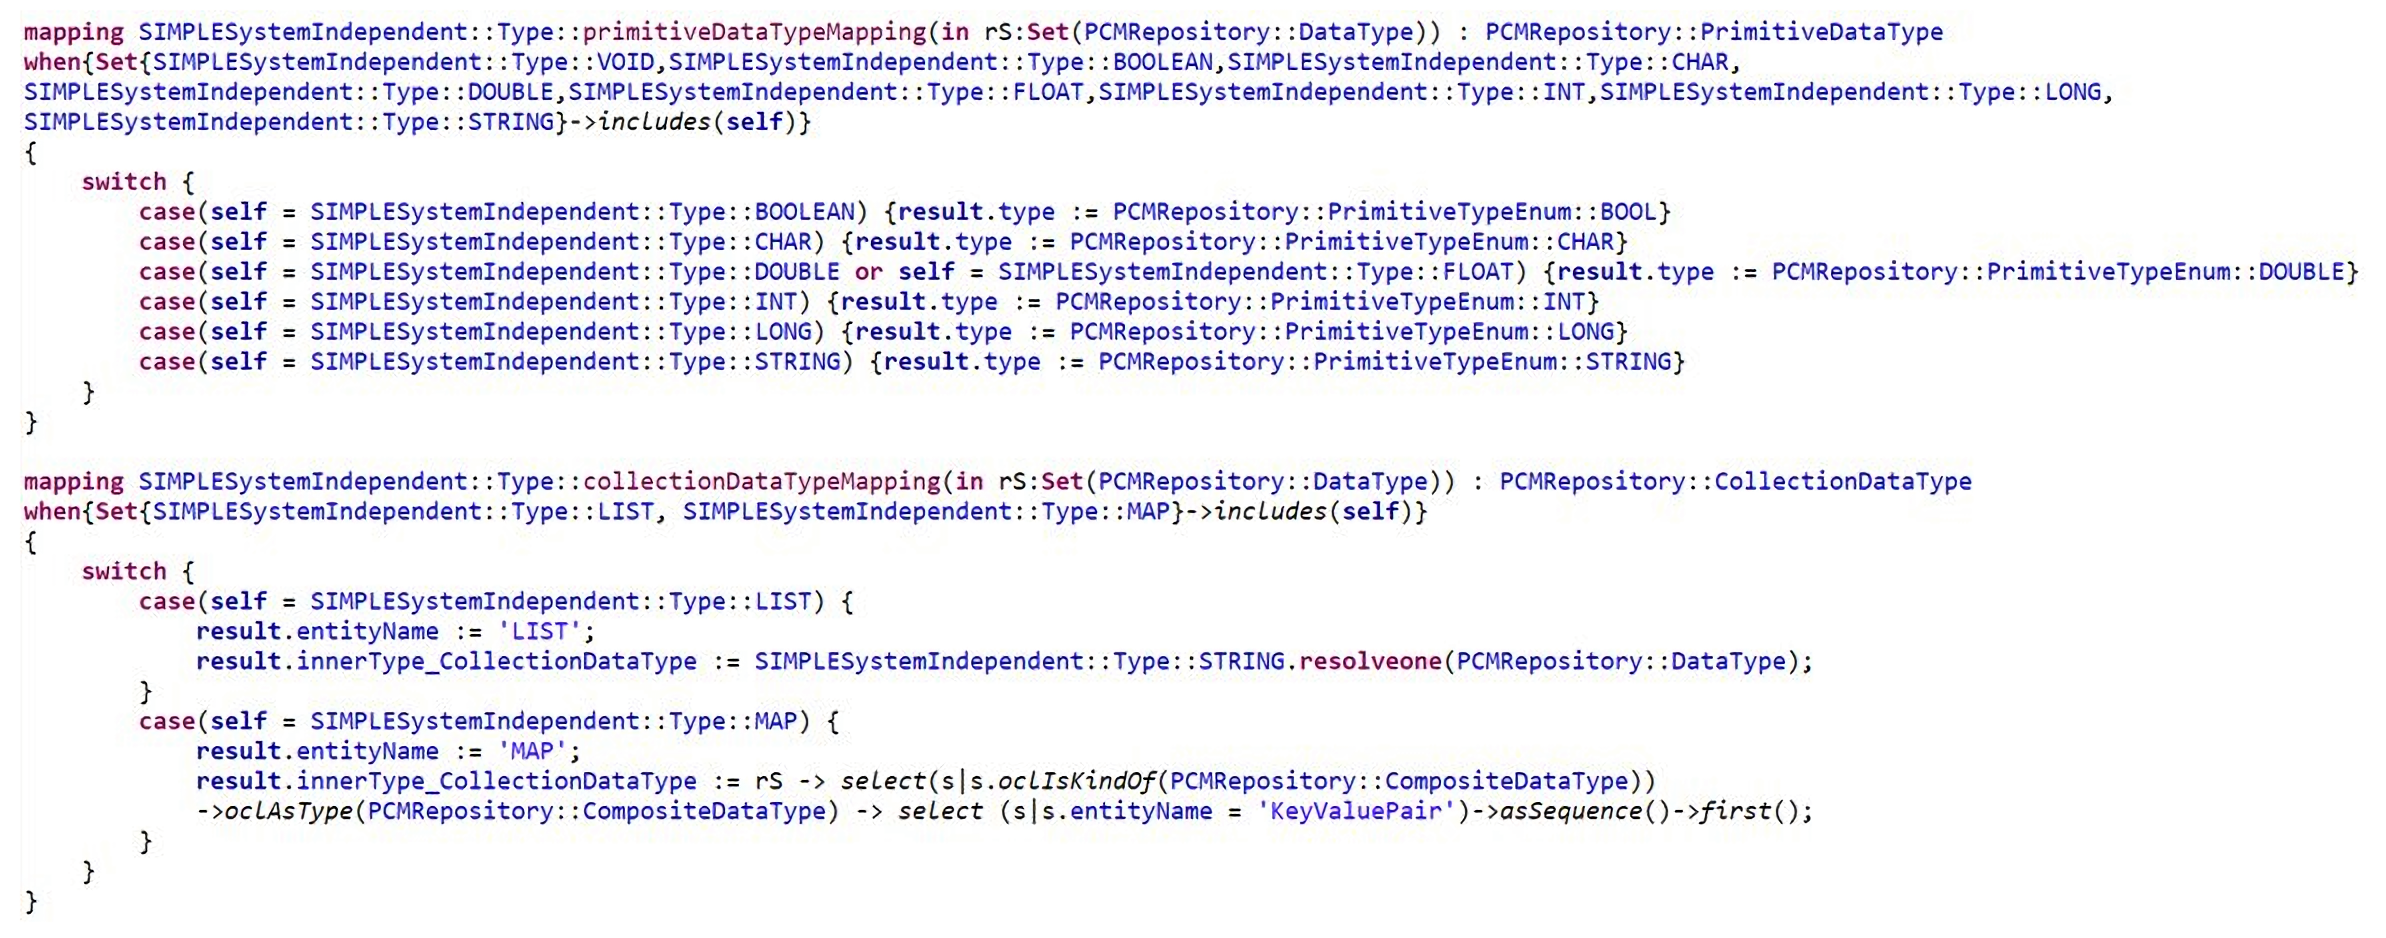
\includegraphics[height=60mm]{figures/modellierung-enum-objekt.png}
\end{frame}

\begin{frame}{Vererbungshierarchien}
	\centering
	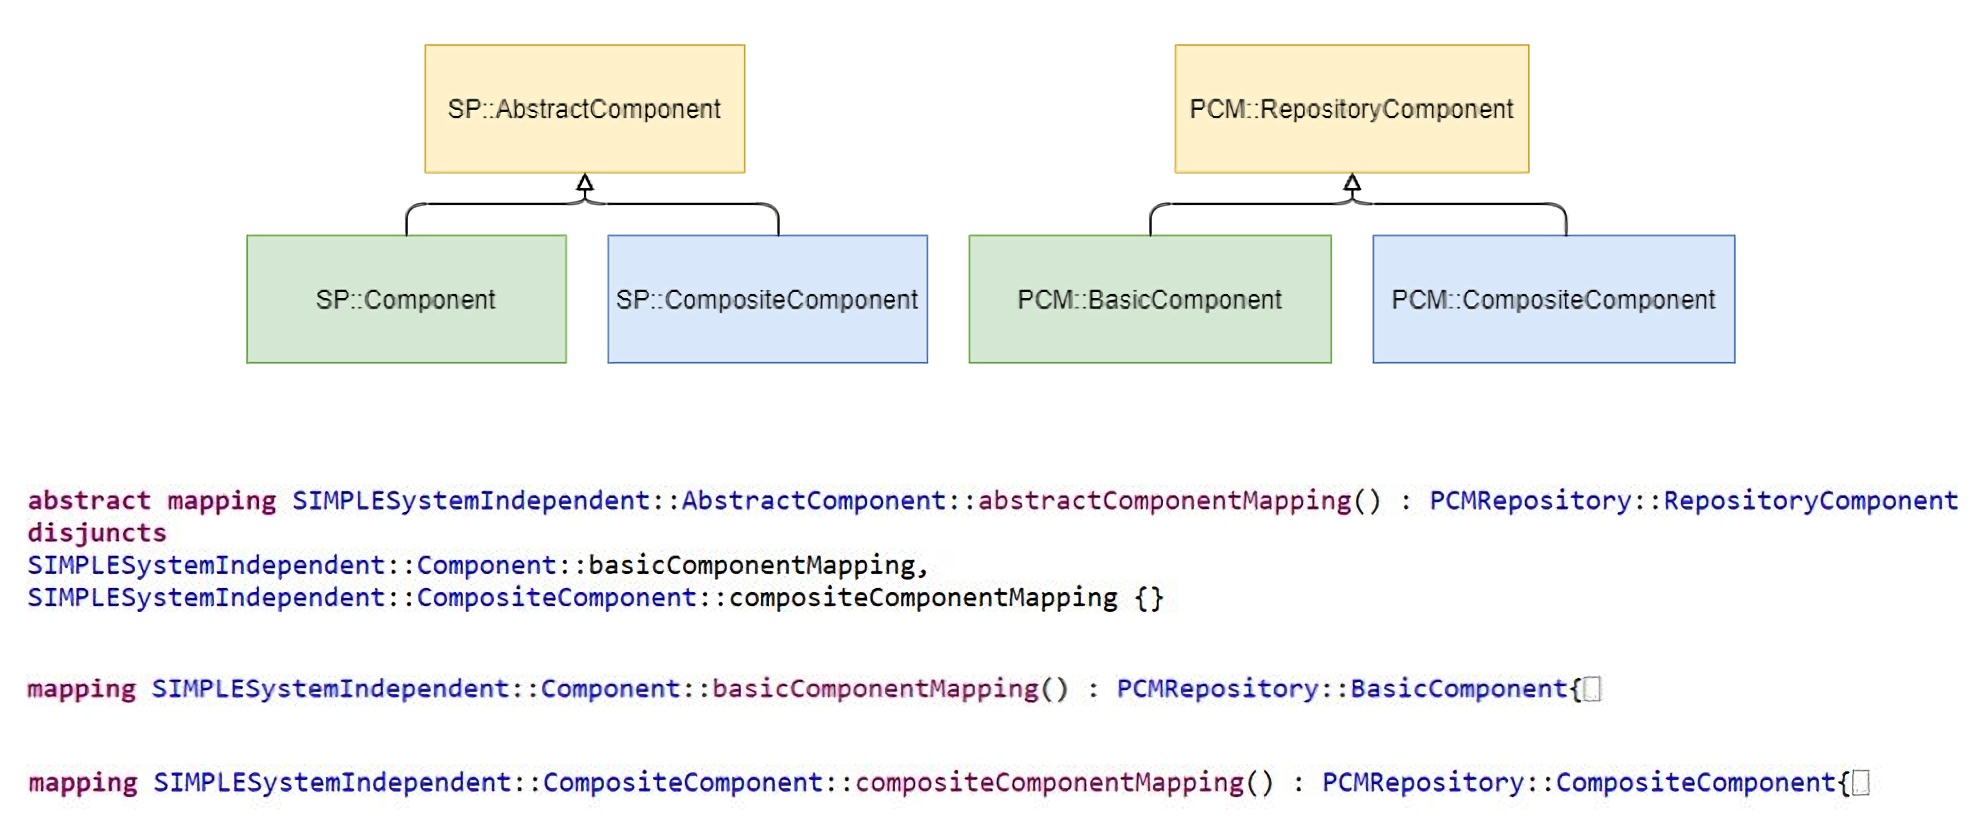
\includegraphics[height=60mm]{figures/vererbungshierachien.png}
\end{frame}

\begin{frame}{Weniger-explizite Informationen}
	\begin{enumerate}
		\item Lösung $\rightarrow$ Intermediate Objekte einführen und diese mappen
	\end{enumerate}
	\centering
	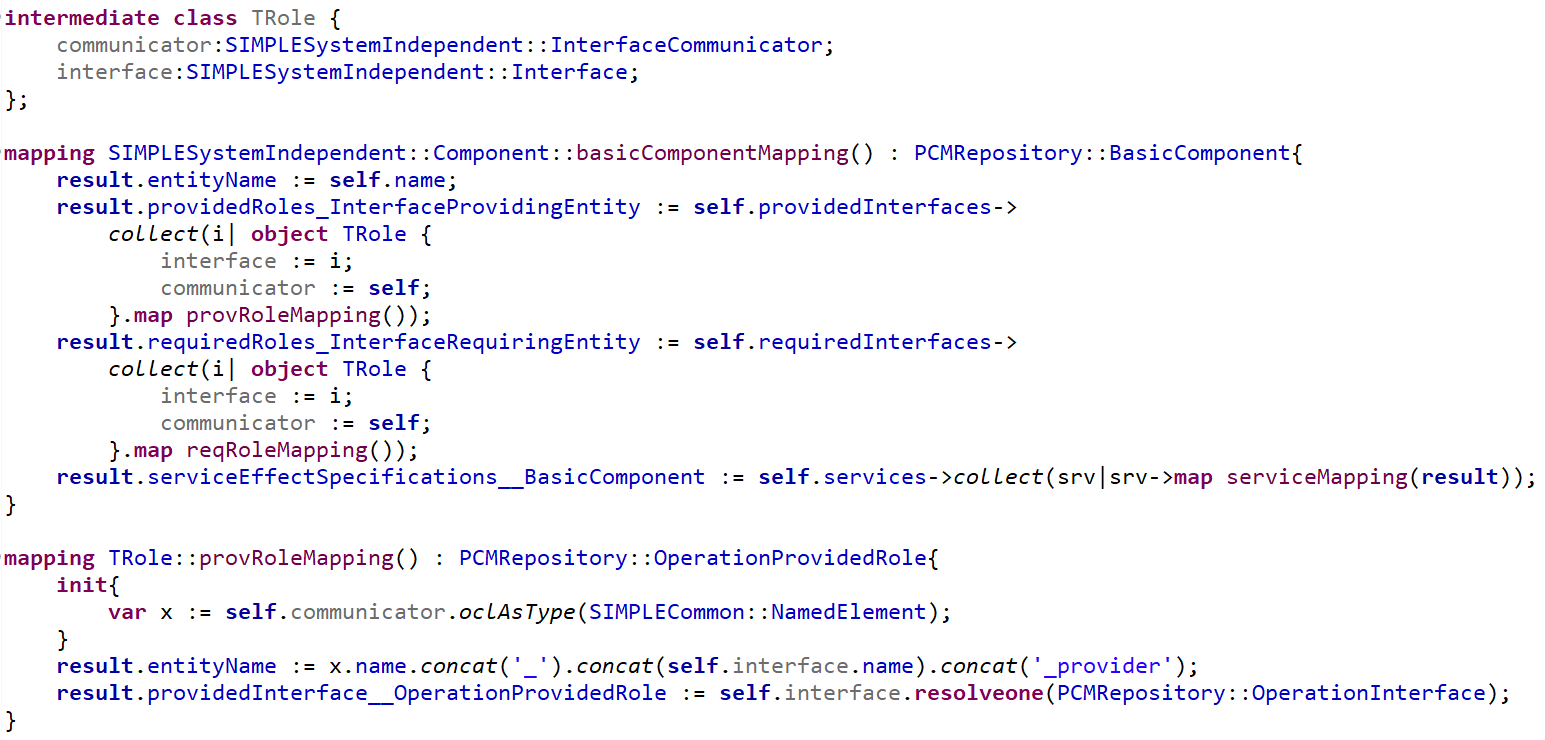
\includegraphics[height=50mm]{figures/intermediate-objekte.png}
\end{frame}